\documentclass[a4paper,12pt]{ctexart}
% Packages
\usepackage{graphicx}
\usepackage{amsmath}
\usepackage{geometry}
\usepackage[ruled,vlined]{algorithm2e}
\usepackage{fancyhdr}
\usepackage{array}
\usepackage{setspace}
\usepackage{titlesec}  % For title formatting
\usepackage{amssymb}
\usepackage{hyperref}
\geometry{margin=1in}
\setstretch{1.5}

% Header and Footer
\pagestyle{fancy}
\fancyhf{}
\fancyhead[L]{Lab Report}
\fancyhead[R]{\thepage}

% Title Formatting
\titleformat{\section}{\normalfont\Large\bfseries}{\thesection}{1em}{}

% Cover Page
\title{
	\vspace{2cm} % Adjust vertical space
	% \includegraphics[width=0.55\textwidth]{logo_hkust2.png} \\ % Add your logo here (change "logo.png" to the actual filename)
	\vspace{1cm} % Adjust vertical space after the logo
	\textbf{\Huge 最优化方法程序作业\\实验报告} \\
	\vspace{1cm} % Adjust vertical space
	% \large Course Code and Name \\
	\vspace{0.5cm} % Adjust vertical space
	% \large {\today}
}
\author{吴羽迪   2300010631}
\date{}

\begin{document}
	
	% Title Page
	\maketitle
	\thispagestyle{empty}
	\newpage
	
	% Table of Contents
	% Start page numbering from the Table of Contents
	\setcounter{page}{1}  % Start counting from 1
	\tableofcontents
	\newpage
	
	\section{问题描述}
	算法需要求解的 Group LASSO 问题为：
	\begin{equation}
		\min_{x \in \mathbb{R}^{n \times l}} \frac{1}{2} \|Ax - b\|_F^2 + \mu \|x\|_{1,2}
		\label{eq.1}
	\end{equation}
	其中$A \in \mathbb{R}^{m \times n}$, $b \in \mathbb{R}^{m \times l}$, $\mu >0$并且
	\[
	\|x\|_{1,2} = \sum_{i=1}^n\|x_{(i,1:l)}\|_2
	\]
	其中$x_{(i,1:l)}$是矩阵$x$的第$i$行。
	
	\section{评价指标}
	项目完成了多个算法的实现。为了实现不同算法效率之间的对比，本项目将使用以下指标来评价各个算法的性能。
	
	\begin{itemize}
		\item \texttt{Err-to-exact}：算法得到的最终目标函数值和最优函数值之间的差的绝对值：
		$$
		\texttt{Err-to-exact}(f_x, f_u) = |f_x - f_u|
		$$
		其中$f_x$为算法得到的最优函数值，$f_u$为实际最优函数值（在本次实验中，$f_u$取为CVX调用Mosek或Gurobi求解器求解此Group Lasso问题时，得到的结果）。
		\item \texttt{Err-to-CVX-Mosek/Gurobi}：算法得到的最终解和最优解之间的归一化范数差：
		$$
		\texttt{Err-to-CVX-Mosek/Gurobi}(x,u) = \frac{\|x - u\|_F}{1 + \|u\|_F}
		$$
		其中$x$为算法得到的最优解，$u$为实际最优解（在本次实验中$u$取为CVX调用Mosek或Gurobi求解器求解此Group Lasso问题时，得到的结果）。
		\item \texttt{Sparasity}：算法得到的最终解的稀疏度：
		$$
		\texttt{Sparasity} = \frac{\|x\|_0}{n \times l}
		$$
		其中$x$为算法得到的最终解，$\|x\|_0$表示x中非零元素的个数。在本项目中认为绝对值小于$10^{-6}$的元素为0。
		\item \texttt{Optval}：算法得到的最终目标函数值。
		\item \texttt{CPU(s)}：算法求解的运行时间。
		\item \texttt{Iter}：算法求解的迭代次数。	
	\end{itemize}
	
	% 3. Methodology/Design Procedures
	\section{问题求解}
	\subsection{CVX直接求解原问题}
	在安装好Mosek和Gurobi求解器后，我们可以直接通过调用Matlab中的CVX工具包，使用这两个求解器进行求解。求解器的运行日志分别保存在\texttt{gl\_cvx\_mosek.txt}和\texttt{gl\_cvx\_gurobi.txt}中，从日志中读取数据后可绘图\ref{fig.1}如下：
	\begin{figure}[htp]
		\centering
		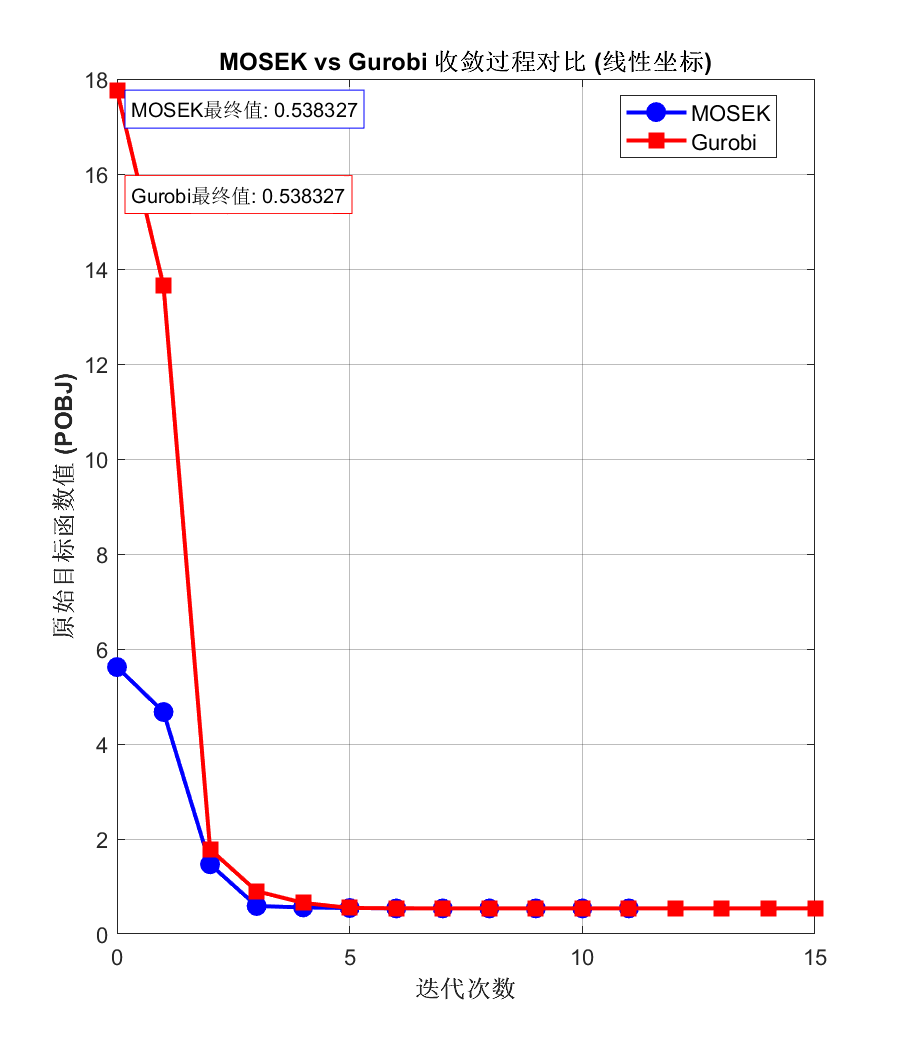
\includegraphics[width=10cm]{img/gl_cvx}
		\caption{mosek和gurobi收敛过程对比}
		\label{fig.1}
	\end{figure}
	
	
	从图\ref{fig.1}以及表\ref{table.1}中可知，使用Mosek求解的迭代次数比使用Gurobi求解的少，但是Gurobi刚开始时收敛的更快，求解的时间也更少。同时，Mosek和Gurobi得到的解在数值上几乎相同，稀疏度也基本一致。
	\subsection{直接调用Mosek和Gurobi求解原问题}
	Mosek和Gurobi有对应的matlab软件包，可以直接调用对应的求解函数进行求解，但需要先将原本的Group Lasso问题转化为函数接口要求的标准形式，如下：			
	$$
	\begin{aligned}
		& \min_{x,t,y,u} \quad u + \mu \sum_{i=1}^{n}t_i \\
		&  \text{s.t.} \qquad Ax - b =y\\
		& \quad \qquad \frac{1}{2}\|y\|_{F}^{2} \le u\\
		& \quad \qquad \|x(i,:)\|_{2} \le t_i, \quad i = 1,\dots, n
	\end{aligned}
	$$
	倘若我们记$x,b,y$的第$i$列分别为$x_i,b_i,y_i(1 \le i \le l)$，并记
	$$
	vec = (x_1^T, \dots, x_l^T, y_1^T, \dots, y_l^T, u, 1, t_1, \dots, t_n)^T \in \mathbb{R}^{M \times 1}
	$$
	其中$M=(n+m)l+n+2$，则上述优化问题可转化为：
	$$
	\begin{aligned}
		& \min_{vec} \quad c^T vec \\
		&  \text{s.t.} \qquad \tilde{A}·vec=-b\\
		& \quad \qquad vec(nl+1:(n+m)l+1) \in \mathcal{Q}^{ml+1}\\
		& \quad \qquad (vec((i-1)l+1:il),vec((n+m)l+2),vec((n+m)l+2+i))\in \mathcal{Q}_r^{l+2} ,\,i = 1,\dots, n
	\end{aligned}
	$$
	其中$\mathcal{Q},\mathcal{Q}_r$分别为二次锥和旋转二次锥，且
	$$
	c = (0,\dots,0,1,0,\mu,\dots,\mu)^T\in \mathbb{R}^{n M \times 1}
	$$
	$$\tilde{A}=(diag{\{-A,\dots,-A\}}, diag{\{I_m,\dots,I_m\}}, \mathbf{0}^{m \times(n+2)})\in \mathbb{R}^{m \times M}
	$$
	此时已经转化为Mosek和Gurobi求解器要求的格式，调用求解器即可完成优化求解，结果如图\ref{fig.2}
	\begin{figure}[htp]
		\centering
		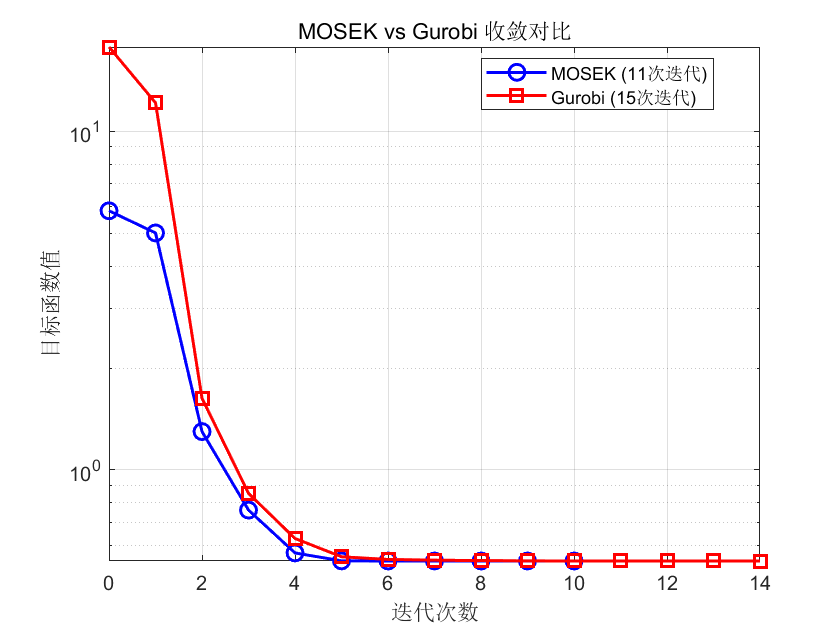
\includegraphics[width=10cm]{img/mosek_gurobi}
		\caption{mosek和gurobi收敛过程对比}
		\label{fig.2}
	\end{figure}\\\\
	由图\ref{fig.2}及表\ref{table.1}可知，直接调用Mosek的求解效率比直接调用Gurobi的更快，迭代次数更少；使用CVX调用两个求解器比直接调用两个求解器用时更长，可能CVX在转换问题形式上消耗了更多时间；直接调用与使用CVX调用在结果以及迭代次数上相差无几。
	\subsection{连续化策略}	
	除了ALM-dual和ADMM-dual，接下来的算法都使用了连续化策略。对于本项目解决的Group Lasso问题，连续化策略从较大的正则化参数$\mu_t$逐步减小到$\mu$（即$\mu_1\ge\dots\ge\mu_{t-1}\ge\mu_{t}\ge\dots\ge\mu$），并求解相应的Group Lasso问题：
	$$
	\min_{x\in\mathbb{R}^{n\times l}}\frac{1}{2}\|Ax-b\|_F^2+\mu_t\|x\|_{1,2}
	$$
	这样做的好处是：在求解$\mu_t$对应的优化问题时，可以利用$\mu_{t-1}$对应的优化问题的解（$\mu_1$子问题使用随机初始点）作为一个很好的逼近解以在较短的时间内完成求解过程；$\mu_t$越大，相应的Group Lasso问题越好解。因此，连续化策略相当于是通过快速求解一系列简单问题来加速求解原始问题。
	
	正则化参数的更新公式为$\mu_{t+1}=max\{\mu_0,\mu_t\eta\}$，其中$\eta\in(0,1)$为缩小因子。在代码实现中，最初的正则化参数是$100\mu$或$1000\mu$，每次乘$0.1$，两或三次后得到$\mu$。
	\subsection{次梯度算法求解原问题}
	次梯度算法的具体流程如下述\textbf{Algorithm \ref{alg:algorithm1}}。需要注意的是，在本项目的代码实践中，倘若某个向量的2-范数小于$1e-6$，我们认为该向量为零向量，并且取它的次梯度为零向量。\newline
	
	\begin{figure}[htp]
		\centering
		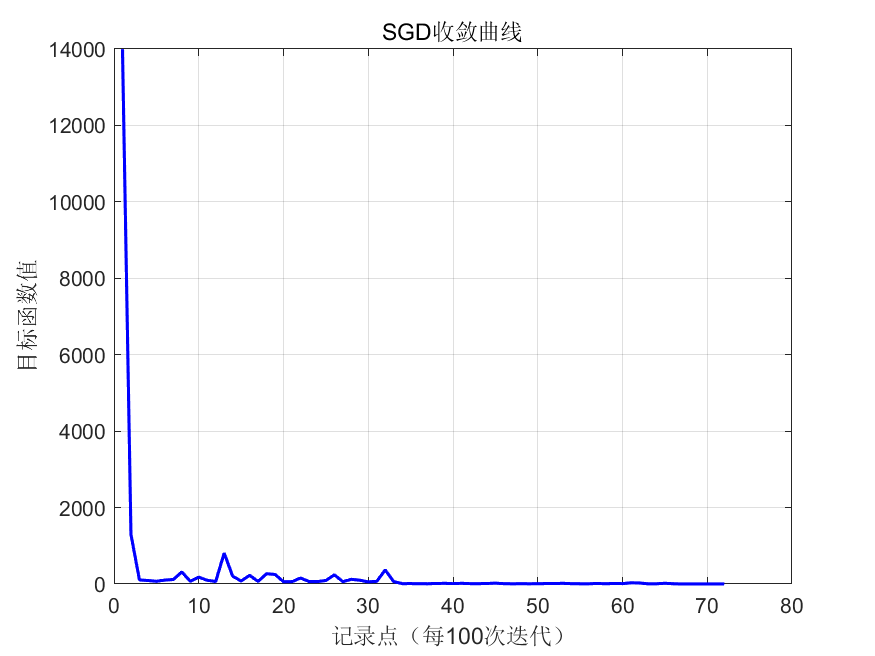
\includegraphics[width=8cm]{img/gl_SGD_primal}
		\caption{SGD收敛过程}
		\label{fig.3}
	\end{figure}
	
	算法中提到的$f^*$为先验的函数最优值，我们使用的是之前mosek求解器求得的函数最优值。
	由表\ref{table.1}和图\ref{fig.3}可知，SGD算法的收敛速度较慢，迭代次数较多，但是每次迭代的时间更短，总用时较为适中。
	此外，相较于其他算法，SGD的收敛曲线较为震荡。这可能是因为步长的选取有时太大，但函数值的曲线最终是收敛到最优值的。
	\begin{algorithm}[!t]
		\label{alg:algorithm1}
		\SetAlgoLined
		\caption{次梯度法}
		\KwIn{$A \in \mathbb{R}^{m\times n},b\in\mathbb{R}^{m\times l},\mu >0$，最大迭代次数$max\_iter$，阈值 $tol>0$，最优函数值$f^*$}
		
		\textbf{Initialize} $x^{(0)}$
		
		\For{$k=0,1,2,\dots,max\_iter$}{
			
				\,\,\,检查停机条件：
				\[
				if\quad {f(x^{(k)})-f^*<tol},\quad break
				\]
				计算次梯度 $g^{(k)}$:
				\[
				g^{(k)} = A^T(Ax^{(k)} - b) + \mu \cdot \partial_{\ell_{1,2}}(x^{(k)})
				\]
				计算步长 $\alpha^{(k)}$:
				\[
				\alpha^{(k)} = \frac{f(x^{(k)})-f^*}{\|g^{(k)}\|_2^2}
				\]
				更新$x^{(k+1)}$:
				\[
				x^{(k+1)}=x^{(k)}-\alpha^{(k)}g^{(k)}
				\]
			
		}
		\Return $x^{(k+1)}$
	\end{algorithm}
	\subsection{梯度下降法求解原问题}
		由于$\|x\|_{1,2}$在$x=0$处是不可微的，我们需要将原本的Group Lasso问题光滑化，这样才能求出梯度，使用梯度下降法。由于对任意的$l$维列向量$x$，有
		$$\|x\|_2=\max_{\|y\|_2 \le 1}y^Tx$$
		所以
		$$\|x\|_{1,2}=\max_{Y\in\mathcal{Y}}\langle x,Y\rangle$$
		其中$\mathcal{Y}=\{Y\in\mathbb{R}^{n\times l}:\, \, \|Y(i,:)\|_2 \le 1,\,\, i=1,2,\dots,n\}$
		
		使用光滑参数$\delta>0$，邻近函数
		$$d(Y)=\frac{1}{2}\|Y\|_F^2=\frac{1}{2}\sum_{i=1}^{n}\|Y(i,:)\|_2^2$$
		记$x_i=x(i,:),y_i=Y(i,:)$，则有
		$$
		\begin{aligned}
			\|x\|_{1,2,\delta}
			&= \max_{Y\in\mathcal{Y}}\langle x,Y\rangle-\,\delta d(Y)\\
			&= \max_{\|y_i\|_2\le 1}\sum_{i=1}^{n}\langle x_i,y_i\rangle-\frac{\delta}{2}\|y_i\|_2^2\\
			&= \sum_{i=1}^{n}\,f_{\delta}(\|x_i\|_2)
		\end{aligned}
		$$
		其中
		$$ f_{\delta}(x)=
		\left\{
		\begin{aligned}
			\frac{t^2}{2\delta},\quad t\le \delta \\
			t-\frac{\delta}{2}, \quad t>\delta 
		\end{aligned}
		\right.
		$$
		原问题(\ref{eq.1})光滑化为
		\begin{equation}
			\min_{x \in \mathbb{R}^{n \times l}} \frac{1}{2} \|Ax - b\|_F^2 + \mu \|x\|_{1,2，\delta}
			\label{eq.2}
		\end{equation}
		其中$\mu$为正则化参数，$\delta$为光滑化参数。对(\ref{eq.2})中的目标函数关于$x$求导，可得梯度矩阵为
		$$g_{\delta}(x)=A^T(Ax-b)+\mu G$$
		其中G的第i行为
		$$
		\frac{\alpha}{\alpha x_i} \|x\|_{1,2,\delta}=
			\left\{
			\begin{aligned}
				\frac{x_i}{\delta},\quad \|x_i\|_2\le \delta \\
				\frac{x_i}{\|x_i\|_2}, \quad \|x_i\|_2>\delta 
			\end{aligned}
			\right.
		$$
		我们使用BB步长进行更新。然而，由于每次构造BB步长需要上一步的数据，所以第一步无法使用BB步长。于是在第一步我们取步长为$\frac{1}{L}$，其中$L=\|A\|_2^2+\frac{\mu}{\delta}$是$g_{\delta}(x)$的$Lipschitz$常数。
		
		下面我们给出具体的算法\textbf{Algorithm \ref{alg:algorithm2}}
		\begin{algorithm}[!t]
			\label{alg:algorithm2}
			\SetAlgoLined
			\caption{梯度下降法}
			\KwIn{$A \in \mathbb{R}^{m\times n},b\in\mathbb{R}^{m\times l},\mu >0$，最大迭代次数$max\_iter$，阈值 $tol>0$，$\delta$的起始与终止值$\delta_{start}>\delta_{final}>0$,递减步数$K$}
			
			\textbf{Initialize} $x^{(0)}$
			
			\For{$k=0,1,2,\dots,K$}{
				$$\delta=\delta_{start}-k\times \frac{\delta_{start}-\delta_{final}}{K}$$
				
				\For{$i=0,1,2,\dots,max\_iter$}{
					
						
						 \,\,\,检查停机条件：
						\[
						if\quad {\|g_{\delta}(x^{(i)})\|_F^2<tol},\quad break
						\]
						 计算步长：
						 
						\If{$i>0$}{
							$$s^{(i-1)}=x^{(i)}-x^{(i-1)}$$
							$$y^{(i-1)}=y^{(i)}-y^{(i-1)}$$
							$$\alpha^{(i)}=\frac{(s^{(i-1)})^Ts^{(i-1)}}{(s^{(i-1)})^Ty^{(i-1)}}$$
						}
						\Else{
							$$\alpha^{(i)}=\frac{1}{\|A\|_2^2+\frac{\mu}{\delta}}$$
						}
						
						 更新$x^{(i+1)}$:
						\[
						x^{(i+1)}=x^{(i)}-\alpha^{(i)}g_{\delta}(x^{(i))}
						\]
					
				}
				$x^{(0)}=x^{(i+1)}$
			}
			\Return $x^{(0)}$
		\end{algorithm}
		，用此算法解决Group Lasso问题时，函数值的变化如图\ref{fig.4}
		\begin{figure}[!t]
			\centering
			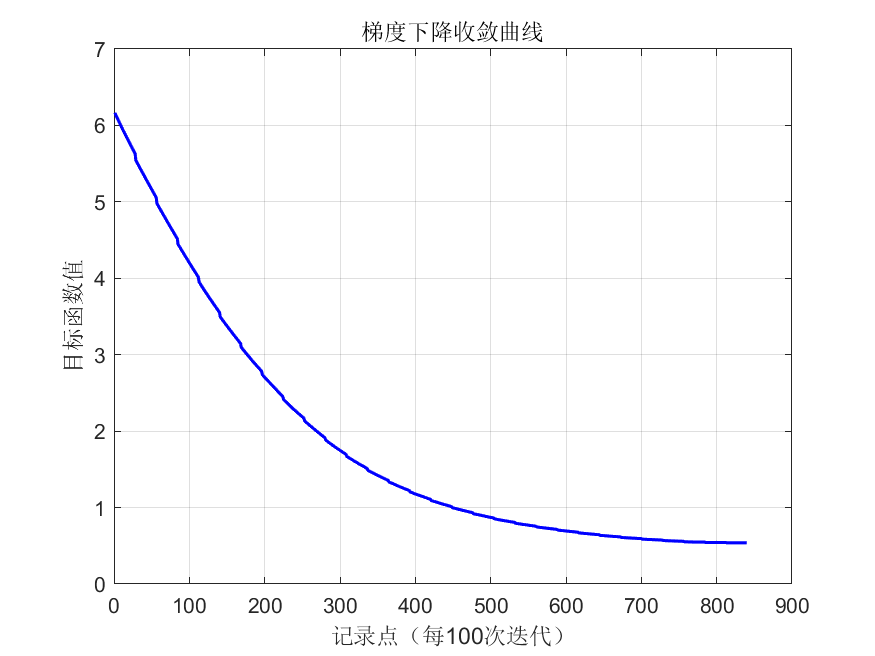
\includegraphics[width=9cm]{img/gl_GD_primal_convergence}
			\caption{GD收敛过程}
			\label{fig.4}
		\end{figure}
		
		从表\ref{table.1}和图\ref{fig.4}中可以看出，梯度下降所用的迭代次数和时间都是最多的。在代码实现的过程中，我发现如果想用梯度下降法更加精确地求解，所需要的时间会大大增加。在权衡取舍下，最终求解出的结果和最优值有一定差距，但是运行时间较为合适。
	\subsection{Nesterov加速梯度下降法求解原问题}
		Nesterov加速梯度下降法几乎相同，只是计算步长的方式不同，算法\textbf{Algorithm \ref{alg:algorithm3}}如下。在此算法中，我们不再采用BB步长，而是采用固定步长$\frac{1}{L}$。用此算法解决Group Lasso问题时，函数值的变化如图\ref{fig.5}。
		\begin{algorithm}[!t]
			\label{alg:algorithm3}
			\SetAlgoLined
			\caption{Nesterov加速梯度下降法}
			\KwIn{$A \in \mathbb{R}^{m\times n},b\in\mathbb{R}^{m\times l},\mu >0$，最大迭代次数$max\_iter$，阈值 $tol>0$，$\delta$的起始与终止值$\delta_{start}>\delta_{final}>0$,递减步数$K$}
			
			\textbf{Initialize} $x^{(0)}$
			
			\For{$k=0,1,2,\dots,K$}{
				$$\delta=\delta_{start}-k\times \frac{\delta_{start}-\delta_{final}}{K}$$
				$$L=\|A\|_2^2+\frac{\mu}{\delta}$$
				\For{$i=0,1,2,\dots,max\_iter$}{
					
					
					\,\,\,检查停机条件：
					\[
					if\quad {\|g_{\delta}(x^{(i)})\|_F^2<tol},\quad break
					\]
					计算步长：
					
					\If{$i>0$}{
						$$\beta^{(i)}=\frac{i-1}{i+2}$$
						$$y^{(i)}=x^{(i)}+\beta^{(i)}(x^{(i)}-x^{(i-1)})$$
						$$x^{(i+1)}=y^{(i)}-\frac{1}{L} \times g_{\delta}(y^{(i)})$$
					}
					\Else{
						$$x^{(i+1)}=x^{(i)}-\frac{1}{L} \times g_{\delta}(x^{(i)})$$
					}
				}
				$x^{(0)}=x^{(i+1)}$
			}
			\Return $x^{(0)}$
		\end{algorithm}
		\begin{figure}[!t]
			\centering
			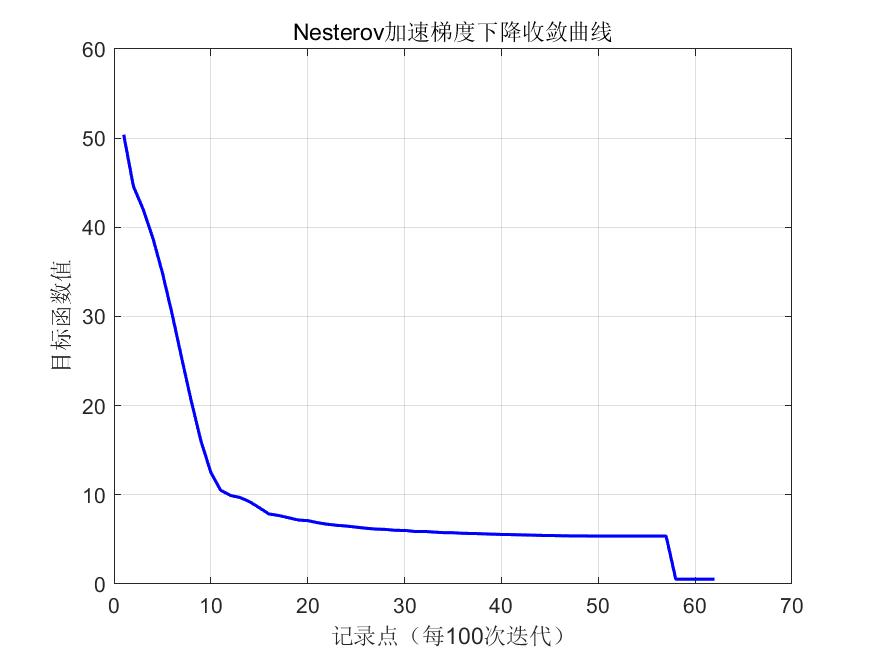
\includegraphics[width=9cm]{img/gl_FGD_primal_convergence}
			\caption{FGD收敛过程}
			\label{fig.5}
		\end{figure}
		
		相较于GD，FGD用时更少，迭代次数也更少，可以适当牺牲时间来得到比GD更精确的结果，如表\ref{table.1}所示。图\ref{fig.5}中下降较快的一个阶梯状部分是$\mu$变小导致的结果。
	\subsection{近似梯度下降法求解原问题}
	对于复合优化问题：
	$$
		\min_x \phi(x)+h(x)
	$$
	其中$\phi$光滑，$h$非光滑。近似点梯度法的迭代格式为
	$$x^{(k+1)}=prox_{t^{(k)}h(·)}(x^{(k)}-t^{(k)}\nabla \phi(x^{(k)}))$$
	这里$t^{(k)}$是步长
	
	在Group Lasso问题中，有
	$$
	\begin{aligned}
	\phi(x)&=\frac{1}{2}\|Ax-b\|_F^2\\
	h(x)&=\mu \|x\|_{1,2}\\
	\nabla \phi(x) &= A^T(Ax-b)
	\end{aligned}
	$$
	下面来求解近似点算子的解析解。近似点算子的定义为
	$$prox_{th}(y)=\arg \min_x\{h(x)+\frac{1}{2t}\|x-y\|_F^2\}$$
	对于$h(x)=\mu\|·\|_{1,2}$，由于惩罚项是逐行可分的，我们可以对每一行独立求解。设$y_i$为输入矩阵的第$i$行（长度为$l$），则需求解
	$$prox_{t\mu\|·\|_2}(y_i)=\arg \min_{x_i}\{\mu\|x_i\|_2+\frac{1}{2t}\|x_i-y_i\|_2^2\}$$
	这是一个凸问题，最优解满足一阶最优性条件。该问题的解为
	$$
	prox_{th}(y_i)=\max (0,1-\frac{t\mu}{\|y_i\|_2})y_i
	$$
	推导如下：
	\begin{itemize}
		\item $x_i\neq0$，目标函数可微。令梯度为零：
		$$\mu\frac{x_i}{\|x_i\|_2}+\frac{1}{t}(x_i-y_i)=0$$
		整理得：
		$$x_i=y_i-\frac{t\mu}{\|x_i\|_2}x_i$$
		由此可得$x_i$与$y_i$同向。设$x_i=\alpha y_i(\alpha\ge0)$，代入上式解得：
		$$\alpha=1-\frac{t\mu}{\|y_i\|_2}$$
		由于要求$\alpha>0$，此时须，满足$\|y_i\|_2>t\mu$。\\
		\item $x_i=0$，次梯度条件为存在$z\in\partial(\|·\|_2)(0)$（即$\|z\|_2\le1$）使得：
		$$0=\mu z-\frac{1}{t}y_i\Rightarrow y_i=t\mu z$$
		因此需满足条件$\|y_i\|_2\le t\mu$
	\end{itemize}
	我们记$L=\|A\|_2^2$，并在近似梯度下降法中取固定步长$\frac{1}{L}$，整理得到的算法\textbf{Algorithm \ref{alg:algorithm4}}如下；
	\begin{algorithm}[!t]
		\label{alg:algorithm4}
		\SetAlgoLined
		\caption{近似梯度下降法}
		\KwIn{$A \in \mathbb{R}^{m\times n},b\in\mathbb{R}^{m\times l},\mu >0$，最大迭代次数$max\_iter$，阈值 $tol>0$}
		
		\textbf{Initialize} $x^{(0)}$
		
		\For{$k=0,1,2,\dots,max\_iter$}{
			
			\,\,\,计算梯度 $g^{(k)}$:
			\[
			g^{(k)} = A^T(Ax^{(k)} - b) 
			\]
			计算近似点算子
			\[
			x_{\text{prox}} = \text{prox}_{\frac{\mu}{L}\lVert \cdot \rVert_{1,2}}\left(x^{(k)} - \frac{1}{L} g^{(k)}\right)
			\]
			更新$x^{(k+1)}$:
			\[
			x^{(k+1)} = x_{\text{prox}}
			\]
			检查停机条件：
			\[
			if\quad {\|x^{(k+1)}-x^{(k)}\|_2<tol},\quad break
			\]
			
		}
		\Return $x^{(k+1)}$
	\end{algorithm}
	用近似梯度下降法解决Group Lasso问题时，函数值的变化如图\ref{fig.6}
	\begin{figure}[!t]
		\centering
		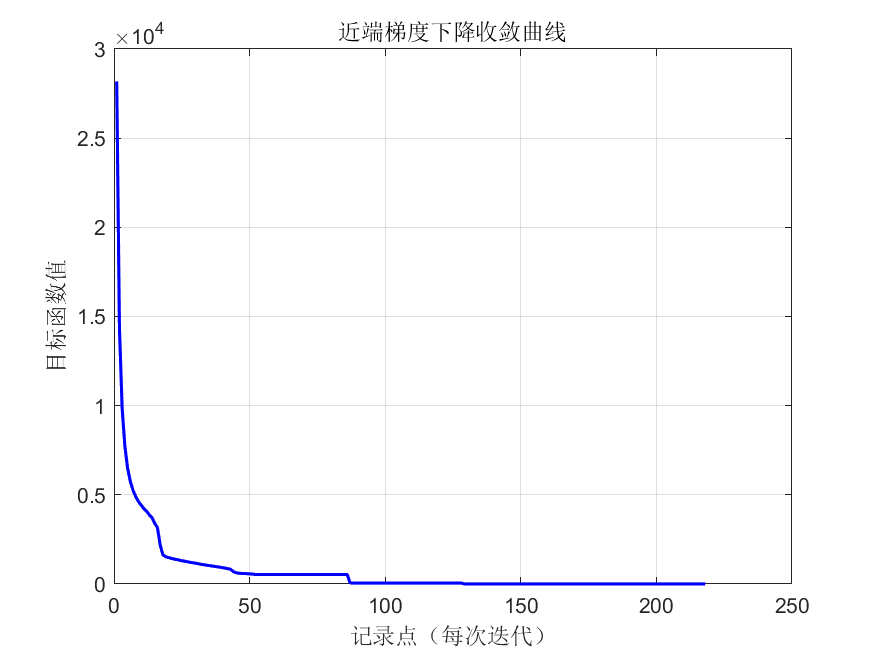
\includegraphics[width=10cm]{img/gl_ProxGD_primal}
		\caption{ProxGD收敛过程}
		\label{fig.6}
	\end{figure}
	
	从表\ref{table.1}中可以看出，相比前面三种梯度下降，ProxGD的求解速度较快，迭代次数较少。从图\ref{fig.6}中可以看出，函数值刚开始时下降极快。这是使用连续化的好处：我们可以先使用较大的$\mu$快速减小函数值。
	\subsection{FISTA求解原问题}
	Nesterov加速近似梯度下降法与近似梯度下降法类似，只是更新的过程稍有不同，给出算法\textbf{Algorithm \ref{alg:algorithm5}}如下，运行结果如图\ref{fig.7}
	\begin{algorithm}
		\label{alg:algorithm5}
		\SetAlgoLined
		\caption{FISTA}
		\KwIn{$A \in \mathbb{R}^{m\times n},b\in\mathbb{R}^{m\times l},\mu >0$，最大迭代次数$max\_iter$，阈值 $tol>0$}
		
		\textbf{Initialize} $x^{(0)}$
		
		\For{$k=0,1,2,\dots,max\_iter$}{
			
			\,\,\,
			计算近似点算子
			\[
			\begin{aligned}
			y^{(k)}&=x^{(k)}+\frac{k-1}{k+2}(x^{(k)}-x^{(k-1)})\\
			g^{(k)} &= A^T(Ay^{(k)} - b) \\
			x_{\text{prox}} &= \text{prox}_{\frac{\mu}{L}\lVert \cdot \rVert_{1,2}}\left(y^{(k)} - \frac{1}{L} g^{(k)}\right)
			\end{aligned}
			\]
			更新$x^{(k+1)}$:
			\[
			x^{(k+1)} = x_{\text{prox}}
			\]
			检查停机条件：
			\[
			if\quad {\|x^{(k+1)}-x^{(k)}\|_2<tol},\quad break
			\]
			
		}
		\Return $x^{(k+1)}$
	\end{algorithm}
	\begin{figure}[!t]
		\centering
		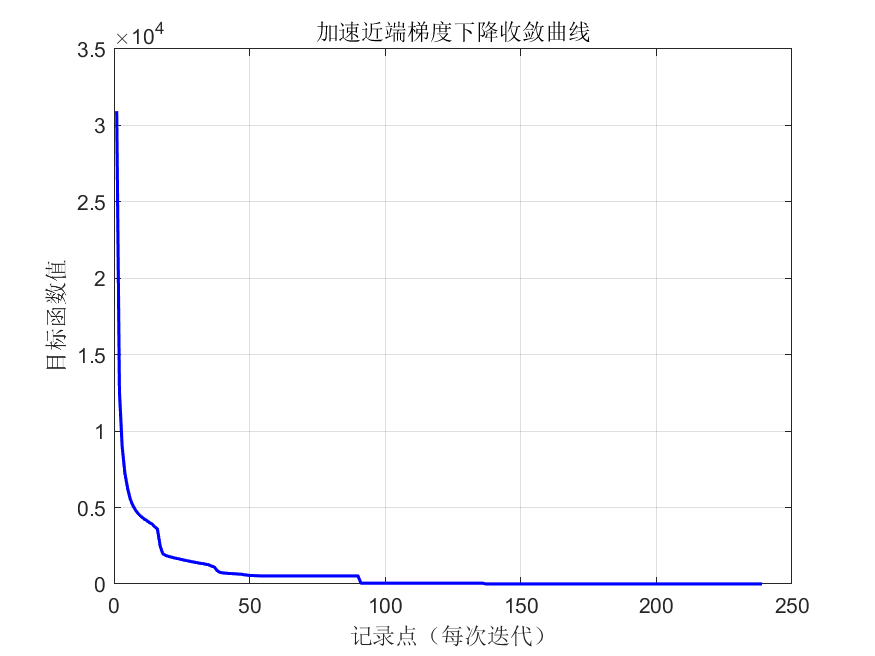
\includegraphics[width=10cm]{img/gl_FProxGD_primal}
		\caption{FProxGD收敛过程}
		\label{fig.7}
	\end{figure}
	
	FProxGD和PorxGD的求解结果相似，相比之下前者用时更短，但所需迭代次数更多。两者的收敛曲线也极为相似，都是一条非常贴近两条坐标轴的曲线。
	\subsection{增广拉格朗日函数法求解对偶问题}
	先给出原问题的对偶问题：
	$$
	\begin{aligned}
		& \min_{z} \quad \frac{1}{2}\|z\|_F^2+\langle b,z\rangle \\
		&  \text{s.t.} \qquad \|(A^Tz)_i\|_2 \le \mu,\,\, i=1,2,\dots ,n
	\end{aligned}
	$$
	其中$(A^Tz)_i$是$A^Tz$的第$i$行（$z$是$m\times l$矩阵，$A^Tz$是$n \times l$矩阵）。引入辅助变量，对偶问题等价于
	$$
	\begin{aligned}
		& \min_{z} \quad \frac{1}{2}\|z\|_F^2+\left< b,z\right> \\
		&  \text{s.t.} \qquad A^Tz=w\\
		& \quad \qquad \|w_i\|_2 \le \mu,\,\, i=1,2,\dots,n
	\end{aligned}
	$$
	引入拉格朗日乘子$\lambda\in\mathbb{R}^{n\times l}$和罚因子$\sigma>0$，作增广拉格朗日函数：
	$$
	L_{\sigma}(z,w,\lambda)=\frac{1}{2}\|z\|_F^2+\langle b,z\rangle+\langle\lambda,A^Tz-w\rangle+\frac{\sigma}{2}\|A^Tz-w\|_F^2,\quad \|w\|_{\infty,2}\le\mu
	$$
	增广拉格朗日函数法的迭代格式为：
	$$ 
	\left\{
	\begin{aligned}
		(z^{k+1},w^{k+1})&=\arg\min_{z,\|w\|_{\infty,2}\le\mu}L_{\sigma_k}(z,w,\lambda^k),\\
		\lambda^{k+1}&=\lambda^k+\sigma_k(A^Tz^{k+1}-w^{k+1}),\\
		\sigma_{k+1}&=\min\{\rho\sigma_k,\bar{\sigma}\}.
	\end{aligned}
	\right.
	$$
	先求第一个式子，当$z^{k+1}=z$固定时，解得$w^{k+1}$为：
	$$
	w^{k+1}=\mathcal{P}_{\|w\|_{\infty,2}\le\mu}(A^Tz+\frac{\lambda^{k}}{\sigma_k})
	$$
	将上式代回第一个式子，并用梯度下降法，可以求得$z^{k+1}$，进而求得$w^{k+1}$。
	此算法的运行结果如图\ref{fig.8}
	\begin{figure}[!t]
		\centering
		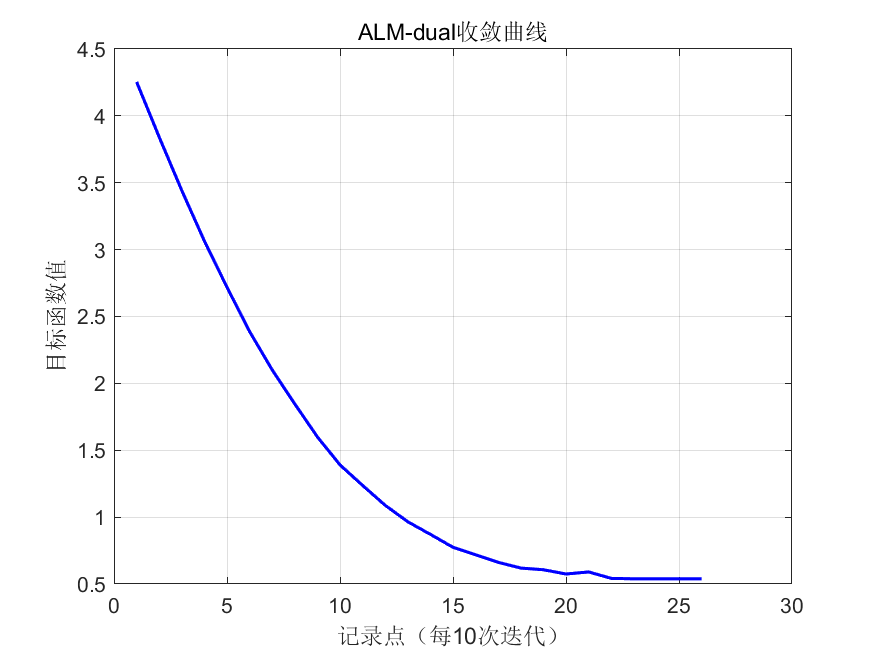
\includegraphics[width=10cm]{img/gl_ALM_dual_convergence}
		\caption{ALM-dual收敛过程}
		\label{fig.8}
	\end{figure}
	
	从表\ref{table.1}中可以看出，ALM-Dual运行所需的时间和迭代次数与前两个近似梯度法相近，但从图\ref{fig.8}可以看出，ALM-dual的收敛曲线并不像前两者一样，在刚开始时快速收敛，这或许是因为ALM-dual并没有使用连续化策略。
	\subsection{交替方向乘子法求解对偶问题}
	先给出原问题的对偶问题：
	$$
	\begin{aligned}
		& \min_{z} \quad \frac{1}{2}\|z\|_F^2+\langle b,z\rangle+\mathbb{I}_{\|w\|_{\infty,2}\le\mu}(w) \\
		&  \text{s.t.} \qquad A^Tz=w\\
	\end{aligned}
	$$
	增广拉格朗日函数为：
	$$
	L_{\rho}(z,w,y)=\frac{1}{2}\|z\|_F^2+\langle b,z\rangle+\mathbb{I}_{\|w\|_{\infty,2}\le\mu}(w)+\langle y,A^Tz-w\rangle+\frac{\rho}{2}\|A^Tz-w\|_F^2
	$$
	
	我们需要在以下几个不同的条件下求解$\min_{w,y,z}L_{\rho}(z,w,y)$，进而得到$w,y,z$的迭代公式：
	
	
	固定$w=w^{(k)},y=y^{(k)}$时，得到
	$$
	z^{(k+1)}=(I_m+\rho AA^T)^{-1}(A(\rho w^{(k)}-y^{(k)})-b)
	$$
	固定$z=z^{(k)},y=y^{(k)}$时，得到：
	$$
	w_i^{(k+1)}=
	\left\{
	\begin{aligned}
		v_i&,\quad \|v_i\|\le \mu \\
		\mu ·\frac{v_i}{\|v_i\|_2}&, \quad \|v_i\|> \mu
	\end{aligned}
	\right.
	$$
	其中$v=A^Tz^{(k+1)}+\frac{1}{\rho}y^{(k)}$。
	
	y的更新为：
	$$
	y^{(k+1)}=y^{(k)}+\rho(A^Tz^{(k+1)}-w^{(k+1)})
	$$
	此算法的运行结果如图\ref{fig.9}
	\begin{figure}[!t]
		\centering
		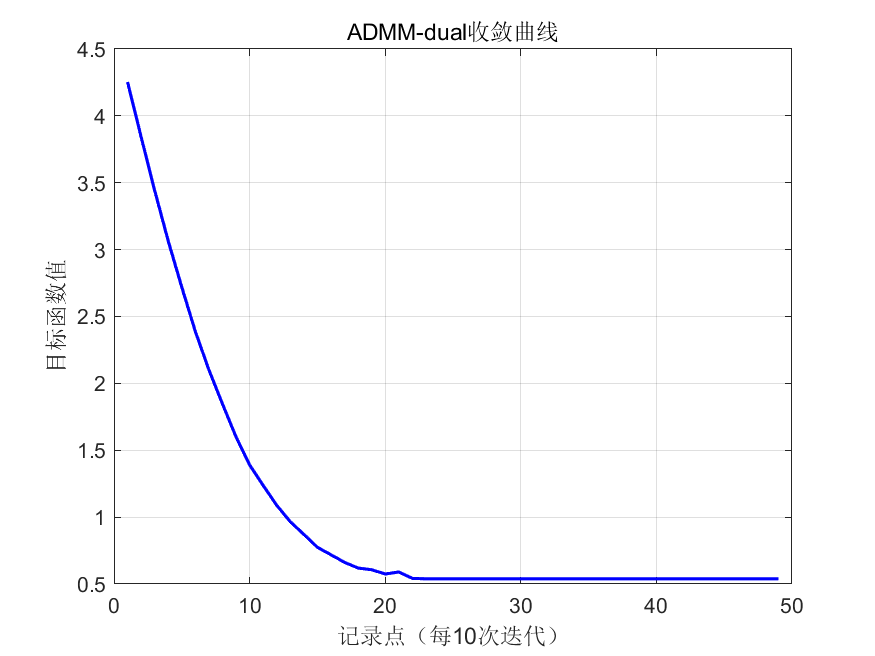
\includegraphics[width=10cm]{img/gl_ADMM_dual_convergence}
		\caption{ADMM-dual收敛过程}
		\label{fig.9}
	\end{figure}
	
	从表\ref{table.1}中可以看出，ADMM-dual与ALM-dual用时相近，但前者所需的迭代次数更多。
	\subsection{交替方向乘子法求解原问题}
	引入辅助变量$z$，原问题转化为：
	$$
	\begin{aligned}
		& \min_{x,z} \quad \frac{1}{2}\|Ax-b\|_F^2+\mu\|z\|_{1,2} \\
		&  \text{s.t.} \qquad x-z=0\\
	\end{aligned}
	$$
	增广拉格朗日函数为：
	$$
	L_{\rho}(x,z,y)=\frac{1}{2}\|Ax-b\|_F^2+\mu\|z\|_{1,2}+\langle y,x-z\rangle+\,\frac{\rho}{2}\|x-z\|_F^2
	$$
	标准ADMM迭代为：
	\begin{itemize}
		\item $x$子问题：
		$$
		\begin{aligned}
		x^{(k+1)}
		=&\arg\min_{x}\frac{1}{2}\|Ax-b\|_F^2+\frac{\rho}{2}\|x-z^{(k)}+\frac{1}{\rho}y^{(k)}\|_F^2\\
		=&(A^TA+\rho I)^{-1}(A^Tb+\rho z^{(k)}-y^{(k)})
		\end{aligned}
		$$
		\item $z$子问题：
		$$
		\begin{aligned}
		z^{(k+1)}
		=&\arg\min_{z}\mu\|z\|_{1,2}+\frac{\rho}{2}\|x^{(k+1)}-z+\frac{1}{\rho}y^{(k)}\|_F^2\\
		=&\,prox_{(\mu/\rho)\|·\|_{1,2}}(x^{(k+1)}+\frac{y^{(k)}}{\rho})\\
		z_i^{(k+1)}=&
		\left\{
		\begin{aligned}
			(1-\frac{\mu}{\rho \|w_i^k\|_2})w_i^k&,\quad \|w_i^k\|_2>\frac{\mu}{\rho} \\
			0&, \quad otherwise
		\end{aligned}
		\right.
		\end{aligned}
		$$
		\item 乘子更新：
		$$
		y^{(k+1)}=y^{(k)}+\rho(x^{(k+1)}-z^{(k+1)})
		$$
	此算法的运行结果如图\ref{fig.10}
	\end{itemize}
		\begin{figure}[!t]
		\centering
		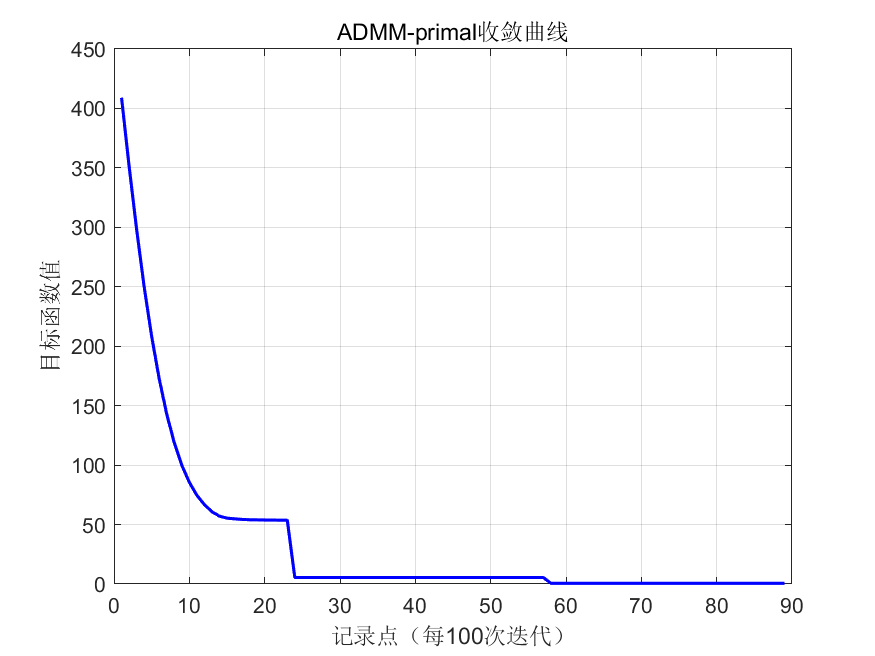
\includegraphics[width=10cm]{img/gl_ADMM_primal}
		\caption{ADMM-primal收敛过程}
		\label{fig.10}
	\end{figure}
	
	从表\ref{table.1}中可以看出，ADMM-primal的迭代次数显著多于ALM-Dual和ADMM-Dual，但运行时间差不多。从图\ref{fig.10}中可以看出，连续化策略使得ADMM-primal在刚开始时快速收敛，$\mu$变小时会出现阶梯状下降。
	\section{实验结果}
	所有算法的运行结果整合在了下面两个表中：
		\begin{table}[h!]
			\begin{center}
				\caption{不同算法的运行结果}
				\label{table.1}
				\begin{tabular}{c|c|c|c|c|c}
					\textbf{Method} & \textbf{CPU(s)} & \textbf{Iter} & \textbf{Optval} & \textbf{Sparsity} & \textbf{Err-to-exact} \\
					\hline
					CVX-Mosek & 9.05 & 11 & 5.38327E-01 & 0.115 &  4.22E-05 \\
					CVX-Gurobi & 4.15 & 15 & 5.38327E-01 & 0.114 &  4.19E-05 \\
					Mosek & 0.34 & 11 & 5.38327E-01 & 0.114 & 4.20E-05 \\
					Gurobi & 0.78 & 14 & 5.38327E-01 & 0.116 & 4.23E-05 \\
					SGD Primal & 1.03 & 7268 & 5.38328E-01 & 0.146 & 5.33E-05 \\
					GD Primal & 13.88 & 86299 & 5.38335E-01 & 0.497 & 5.90E-05 \\
					FGD Primal & 2.71 & 6283 & 5.38327E-01 & 0.117 & 4.28E-05 \\
					ProxGD Primal & 1.74 & 218 & 5.38327E-01 & 0.114 & 4.20E-05 \\
					FProxGD Primal & 1.30 & 239 & 5.38327E-01 & 0.114 & 4.20E-05 \\
					ALM Dual & 1.36 & 260 & 5.38327E-01 & 0.100 & 6.86E-05 \\
					ADMM Dual & 0.93 & 497 & 5.38328E-01 & 0.100 & 5.02E-05 \\
					ADMM Primal & 1.22 & 9126 & 5.38327E-01 & 0.114 & 4.20E-05 \\			
				\end{tabular}
			\end{center}
		\end{table}
		\begin{table}[h!]
			\begin{center}
				\caption{不同算法的精度}
				\label{table.2}
				\begin{tabular}{c|c|c}
					\textbf{Method} & \textbf{Err-to-CVX-Mosek} & \textbf{Err-to-CVX-Gurobi}\\
					\hline
					CVX-Mosek & 0.00E+00 & 3.76E-07 \\
					CVX-Gurobi & 3.76E-07 & 0.00E+00 \\
					Mosek & 2.41E-07 & 1.44E-07  \\
					Gurobi & 2.43E-07 & 5.73E-07 \\
					SGD Primal & 1.45E-05 & 1.48E-05 \\
					GD Primal & 1.91E-05 & 1.94E-05 \\
					FGD Primal & 8.19E-07 & 1.03E-06 \\
					ProxGD Primal & 3.47E-07 & 5.01E-08 \\
					FProxGD Primal & 3.42E-07 & 5.50E-08 \\
					ALM Dual & 3.19E-05 & 3.21E-05 \\
					ADMM Dual & 1.07E-05 & 1.09E-05 \\
					ADMM Primal & 3.51E-07 & 6.46E-08 \\			
				\end{tabular}
			\end{center}
		\end{table}
	\section{参考资料}
	【1】\,文再文老师的课程讲义与课程主页
	http://faculty.bicmr.pku.edu.cn/~wenzw/opt-2025-fall.html
	
	【2】\,程序作业提交指南 http://faculty.bicmr.pku.edu.cn/~wenzw/opt2015/homework5-req.pdf
	
	【3】\,李锦韬学长的仓库
	https://github.com/AkexStar/Algorithms-group-LASSO-problem
	
	【4】王晨宇学长的仓库
	https://github.com/cwangPKU/Optimization\_Algorithms
\end{document}